\chapter{Literature Review}
\label{LitReview}

\section{Colour Science}

\subsection{Illumination and Colour Vision}

Organisms on earth posses visual systems such that they can glean information about spatially remote objects through the sensing of light reflected from these objects to the organism. They are able to do this because the sun emits electromagnetic radiation (which we call `light' when it is within our visual sensitivity range) our atmosphere transmits many parts of this radiation (absorbing some, more-so of some wavelengths than others), and objects reflect this radiation (again, absorbing some, more-so of some wavelengths than others).
%minnaert

\begin{figure}[htbp]
%\includegraphics[max width=\textwidth]{figs/litReview/???.png}
\caption{The \gls{SPD} of the sun, filtered through our atmosphere, daylight reaching the ground (sunlight plus scattered blue-sky light) and reflected from 2 different surfaces}
\label{fig:SPD}
\end{figure}

Our perception of colour generally correlates with the way in which objects preferentially reflect some wavelengths over others (described by the \acrfull{SRF}) which assists in the recognition of objects (that's a banana) and the discrimination of distinct objects, often in a manner that it ecologically beneficial (that's a \emph{ripe} banana).

\subsection{Chromatic Adaptation and Colour Constancy}
`Adaptation' is the general mechanism by which a finite range of sensitivity can be shifted in terms of absolute sensitivity bounds. The benefit of having an adaptive system, as opposed to a fixed system, is that the sensitivity of the system to small changes is maximised, whilst maintaining a broad overall sensitivity, at the expense of being able to sense over the entire range at a single time-point. 

\begin{figure}[htbp]
%\includegraphics[max width=\textwidth]{figs/litReview/???.png}
\caption{A comparison between a system with fixed sensitivity vs. one with an adaptive sensitivity.}
\label{fig:adaptation}
\end{figure}

In an environment such as the terrestrial environment, there is a great range in the level of illumination, but this range is rarely existent contiguously; levels of illumination tend to similar across a scene, and only change rather slowly. The notable exception, and thus where we notice the expense of having an adaptive visual system, comes when we enter or exit an environment where illumination is almost entirely excluded, such as a dark cave or below decks of a boat. 

Where the process of adaptation responds to overall illumination levels, it is referred to as light adaptation and dark adaptation. 

Chromatic adaptation

Colour constancy

\subsubsection{Colour Constancy Research}

\subsection{Colorimetry and Colour Measurement}

\textit{The current recommended source for colorimetry is CIE 015:2018 \citep{cie_cie_2018}\footnote{Though as \citet{fairchild_cie_2019} notes, this document is `expensive and somewhat difficult to find', and as such I have been using a draft of the now superseded \citet{cie_cie_2004-2}.}. My personal opinion is that an understanding of colorimetry of CIE colorimetry is best gained from an understanding of it's history, and for this I recommend Janos Schanda's book `Colorimetry: Understanding the CIE System'\citep{schanda_colorimetry_2007}.}

\bigskip

Colorimetry is the study of the quantitative specification of colour. As a subjective, internal and anthropocentric concept, in order to measure anything meaningful and comparable, we use a standard observer, or more precisely, one of a number of defined standard observers \cite{cie_bs_2011}.

The classic standard observer was defined by the CIE in 1931, following experiments by Wright and Guild \cite{wright_re-determination_1929, guild_colorimetric_1931}. Despite several more recently published standard observers, the 1931 observer is still much used, and I shall use it in the following example of how a basic colorimetric computation is performed.

An illuminant is defined by its \gls{SPD}, a surface as it's \gls{SRF}, and a the sensitivity of a sensor (such as a photosensitive cell in the retina, or a pixel in a camera) by its \gls{CMF} (or in the case that biologically based measurements are used - the \gls{SSF}).

\begin{figure}[htbp]
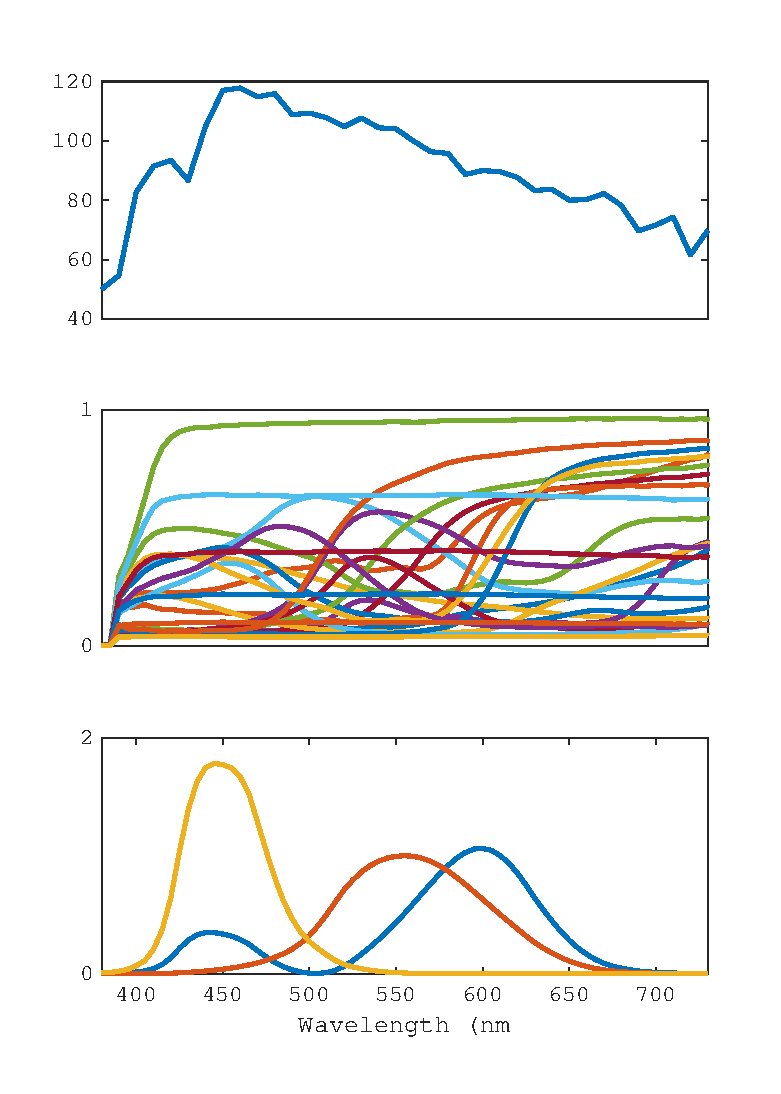
\includegraphics[max width=\textwidth]{figs/LitRev/SPDetc.pdf}
\caption{A \gls{SPD}, a set of \glspl{SRF} and three \glspl{CMF}.}
\label{fig:specFun}
\end{figure}

The light reaching the eye for a given reflecting surface under a given illuminant (termed the `colour signal') can be computed by multiplying the \gls{SPD} by the \gls{SRF} at each sampled interval.

\begin{equation}
\phi(\lambda)=R(\lambda) \cdot S(\lambda)
\end{equation}

Explain\dots \\
From this tristimulus values can then be computed.

\begin{subequations}
\begin{align}
X=k \sum_{\lambda} \phi_{\lambda}(\lambda) \overline{x}(\lambda) \Delta \lambda \\ 
Y=k \sum_{\lambda} \phi_{\lambda}(\lambda) \overline{y}(\lambda) \Delta \lambda \\ 
Z=k \sum_{\lambda} \phi_{\lambda}(\lambda) \overline{z}(\lambda) \Delta \lambda
\end{align}
\end{subequations}

Explain\dots \\
Following this chromaticity co-ordinates can be computed.

\begin{subequations}
\begin{align}
x=\frac{X}{X+Y+Z} \\
y=\frac{Y}{X+Y+Z} 
\end{align}
\end{subequations}

Explain\dots \\
Here's a \gls{MATLAB} example, using \gls{PTB} for data:

\begin{lstlisting}[language=MATLAB]
load spd_D65     % SPD: CIE D-series illuminant D65
load sur_macbeth % SRF: macbeth colour checker
load T_xyz1931   % CMF: 1931 2deg 

colourSignal = sur_macbeth.*spd_D65;
XYZ = T_xyz1931*colourSignal;
xy = [XYZ(1,:)./sum(XYZ);XYZ(2,:)./sum(XYZ)];
\end{lstlisting}

Plotting: 

\begin{lstlisting}[language=MATLAB]
spectralLocus = [T_xyz1931(1,:)./sum(T_xyz1931);T_xyz1931(2,:)./sum(T_xyz1931)];
sRGBSpectralLocus = XYZToSRGBPrimary(T_xyz1931);

figure, hold on, 
scatter(spectralLocus(1,1:70),spectralLocus(2,1:70),[],sRGBSpectralLocus(:,1:70)','filled')
scatter(xy(1,:),xy(2,:),'k')
axis equal, axis([0 1 0 1])
xticks([0 1]), yticks([0 1])
xlabel('x'), ylabel('y')
\end{lstlisting}

\begin{figure}[htbp]
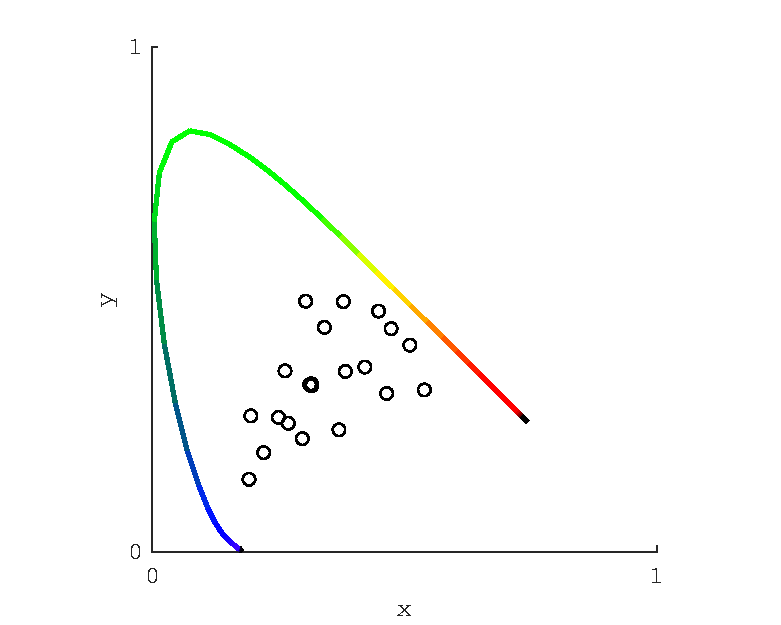
\includegraphics[max width=\textwidth]{figs/LitRev/ColorimetryDemo1.pdf}
\caption{The CIE 1931 chromaticity diagram, with the chromaticity of the macbeth colour checker patches under D65}
\label{fig:1931}
\end{figure}







\subsection{Colour rendering and light quality specification}

\section{Museum Lighting}
\subsection{Current practise in specifying museum lighting}
\subsection{Balancing conservation with observation}
\subsection{Damage factors}
\subsection{LEDs in museums}
\subsection{New opportunities with solid state lighting}


\section{Intrinsically Photosensitive Retinal Ganglion Cells}
\section{Research questions and hypothesese}
